\documentclass[11pt]{article}

\usepackage{amsmath, amssymb}
\usepackage{geometry}
\usepackage{graphicx}
\usepackage{bm}
\usepackage{tikz}
\usetikzlibrary{positioning}
\usepackage{hyperref}
\usepackage{titlesec}

\geometry{margin=2.5cm}
\setlength{\parskip}{6pt}
\setlength{\parindent}{0pt}

\title{\textbf{Symbiotic Insight Framework (SIF)}\\
\large A Structured Method for Stabilising High-Velocity Insight}
\author{Morten Magnusson}
\date{DOI: \href{https://doi.org/10.6084/m9.figshare.30656351}{10.6084/m9.figshare.30656351}}

\begin{document}

\maketitle

\begin{abstract}
This document presents the Symbiotic Insight Framework (SIF), a research method developed within the Energy-Flow Cosmology (EFC) project. SIF describes how high-velocity, cross-domain conceptual insight can be stabilised, organised, and transformed into reproducible scientific structure through continuous interaction between a human thinker and an adaptive computational system.

SIF is neither a psychological theory nor an AI-assistant workflow. It is a practical architecture for managing large-scale scientific structure produced through parallel, field-based reasoning. The framework shows how insight is externalised, refined, semantically integrated, and version-locked in a continuous, self-correcting loop.
\end{abstract}

\section{Summary}

SIF consists of three components:

\subsection{1. Human Contribution}
Insight emerges in parallel conceptual fields rather than linear chains. These fields evolve rapidly and span several domains simultaneously.

Key features:
\begin{itemize}
    \item parallel conceptual fields
    \item rapid formation of large-scale structures
    \item cross-domain integration
    \item continuous pattern recognition
\end{itemize}

\subsection{2. System Contribution}
The system stabilises and organises the structures generated by the human participant.

Key features:
\begin{itemize}
    \item structural consolidation
    \item semantic indexing
    \item cross-file and cross-domain continuity
    \item versioned documentation
    \item automated validation
\end{itemize}

\subsection{3. Symbiotic Field}
Insight is produced in the interaction between human and system. The human drives conceptual shifts; the system stabilises the structure. Neither produces the scientific output alone.

\section{Methodology}

The SIF process follows a clear cycle:

\begin{enumerate}
    \item \textbf{Insight generation:} rapid, high-order conceptual patterns emerge in parallel.
    \item \textbf{Immediate externalisation:} raw insight is captured before structural decay.
    \item \textbf{Structural refinement:} the system returns a coherent, navigable structure.
    \item \textbf{Semantic integration:} concepts are linked across domains using JSON-LD, schema, and index maps.
    \item \textbf{Version locking:} outputs are stabilised using DOIs, metadata, and reproducible pipelines.
    \item \textbf{Iterative reinforcement:} the loop generates new insight which is stabilised again.
\end{enumerate}

This creates a self-consistent and self-documenting research environment.

\section{Role in the EFC Project}

SIF supports and stabilises:
\begin{itemize}
    \item the structure of the Energy-Flow Cosmology theory
    \item repository organisation and file hierarchy
    \item semantic schema and automated pipelines
    \item cross-domain integration across cosmology, thermodynamics, cognition, and information theory
\end{itemize}

\section{Why This Matters}

SIF demonstrates a new form of scientific workflow where:
\begin{itemize}
    \item large conceptual transformations
    \item cross-domain reasoning
    \item high-density insight
    \item continuous computational structuring
\end{itemize}
operate as one integrated system.

\newpage
\section{Figures}

\subsection*{Figure 1: Core SIF Architecture}

\begin{center}
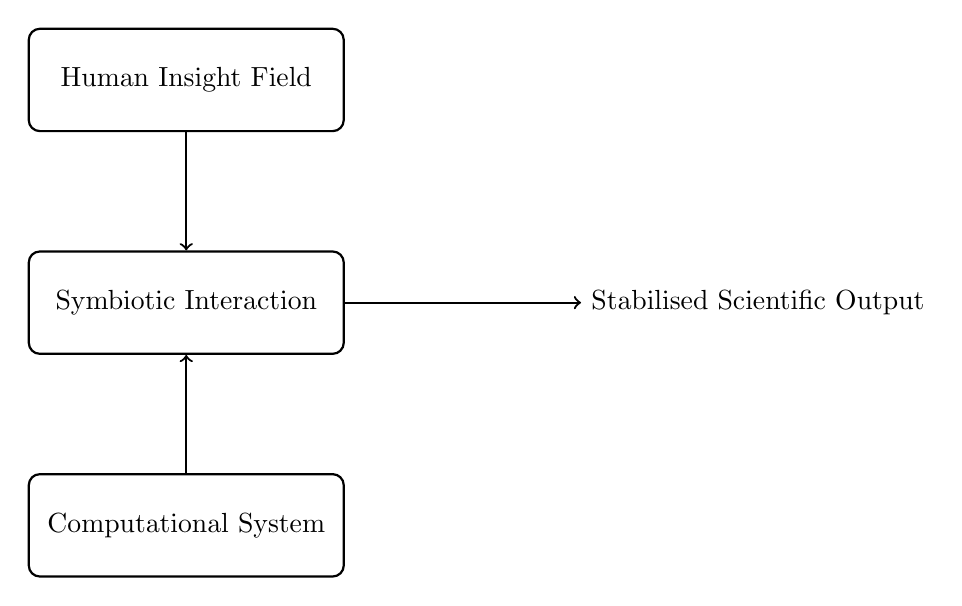
\begin{tikzpicture}[
    box/.style={
        rectangle, rounded corners,
        draw=black, thick,
        text centered,
        minimum width=4cm,
        minimum height=1.3cm
    }
]

\node[box] (human) {Human Insight Field};
\node[box, below=1.5cm of human] (sym) {Symbiotic Interaction};
\node[box, below=1.5cm of sym] (system) {Computational System};

\draw[->, thick] (human) -- (sym);
\draw[->, thick] (system) -- (sym);
\draw[->, thick] (sym.east) -- ++(3,0) node[right]{Stabilised Scientific Output};

\end{tikzpicture}
\end{center}

\subsection*{Figure 2: SIF Process Loop}

\begin{center}
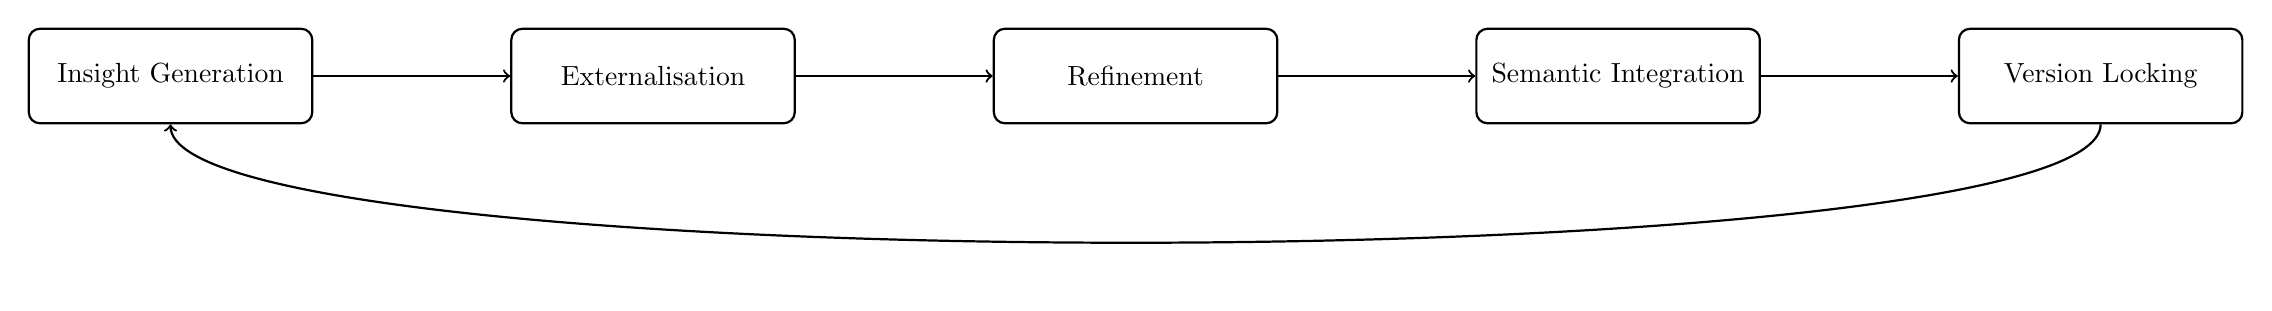
\begin{tikzpicture}[
    stepbox/.style={
        rectangle, rounded corners,
        draw=black, thick,
        minimum width=3.6cm,
        minimum height=1.2cm,
        text centered
    }
]

\node[stepbox] (ins) {Insight Generation};
\node[stepbox, right=2.5cm of ins] (ext) {Externalisation};
\node[stepbox, right=2.5cm of ext] (ref) {Refinement};
\node[stepbox, right=2.5cm of ref] (sem) {Semantic Integration};
\node[stepbox, right=2.5cm of sem] (ver) {Version Locking};

\draw[->, thick] (ins) -- (ext);
\draw[->, thick] (ext) -- (ref);
\draw[->, thick] (ref) -- (sem);
\draw[->, thick] (sem) -- (ver);
\draw[->, thick] (ver.south) .. controls +(0,-2) and +(0,-2) .. (ins.south);

\end{tikzpicture}
\end{center}

\section{Keywords}

symbiosis, methodology, insight process, human--system workflow, semantic organisation, large-scale structure, cognitive integration, EFC, meta-architecture

\end{document}
